\documentclass[12pt, letterpaper]{report}
\usepackage[margin=1in]{geometry}
\usepackage[utf8]{inputenc}
\usepackage{url}
\usepackage{hyperref}
\usepackage{graphicx}

\title{\Huge Guia de seguran\c{c}a para leigos}
\author{Gilgamesh}

\begin{document}
\maketitle
\pagebreak
\section*{Espionagem em massa - Um problema mundial}
\large Um dos maiores problemas na nossa sociedade moderna é a espionagem em masas. Governos roubam os teus dados, lhe espionagem e ainda dizem que é para o seu próprio bem.\\

	Depois dos vazamentos (leaks) feito por \textbf{Edward Snowden}, várias pessoas em todo o mundo passaram a se preocupar com a prórpia segurança e privacidade. Mas ainda assim, uma boa parcela da população não se preocupa com a própria privacidade e segurança, muitas vezes por não saber o que governos e empresas fazem com os dados coletados. Mas a população deveria sim se  preocupar com a privacidade, pois os mesmos métodos utilizado pelos governos para roubarem dados, também são utilizado por criminosos.\\

	A espionagem em massa acontece em todo e qualquer lugar do globo, não importa aonda você esteja, se tem algum meio de comunicação você está vulnerável à espionagem. Mesmo que você apenas utilize um telefone fixo, você está vulnerável à espionagem.\\

	As redes sociais atualmente é um dos maiores perigos para a segurança e privacidade dos usuários, visto que é possível determinar os seus gostos, seus amigos, sua família e diversas outras coisas. Sites como o Facebook, enquanto você o utiliza ele monitora o que você está acessando para poder lhe fazer propagandas direcionadas. O Google também faz isto. Embora seja a forma que estas empresas tem de ganhar dinheiro, é muito invasivo e na maioria das vezes não funciona. Mas para poder escapar desta vigilância, tem algumas coisas que podemos fazer.\\
	\begin{itemize}
		\item Utilize o redes sociais apenas quando necessário.
		\item Sempre que for utilizar alguma rede social, utilize-a com alguma VPN.
		\item Se não for necessário ter uma rede social, não tenha.
	\end{itemize}
\pagebreak
%Segurança na internet.
\section*{Segurança na internet}
	A internet é um lugar vasto, mas com vários perigos. Estamos na era da informação, na qual tudo (ou quase tudo) é feito pela internet, e justamente por isso que ela se tornou extremamente perigosa para usuários leigos. Os perigos que corremos não é apenas por criminosos, mas também pelo estado.\\

	Um dos maiores perigos que temos são os ataques de \href{https://criptowiki.miraheze.org/wiki/Phishing}{phishing}, que consiste basicamente em uma clonagem de sites feitos na rede interna ou não e que tem como objetivo roubar dados do usuário, como login e senha de bancos e de redes sociais.\\

	Mas os ataques de phishing tem alguns erros na qual é possível usuários identificarem se estão em um site falso. Um método de verificar se o site é falso ou não, é através da URL (endereço) do site, que \textbf{pode} estar errada e assim o usuário poderá saber se está sendo vítima de um ataque phishing. Então a dica é ficar atento à URL do site.\\

	E uma outra forma além de verificar o endereço URL é verificar o \textbf{certificado SSL}, que é basicamente um protocolo de rede que garante que o site é verídico e que é utilizado junto ao protocolo \textbf{HTTPS}. Em casos de phishing na rede interna, quando o indivíduo invade a rede WiFi, é possível verificar o certificado SSL. Quando você acessar um site de banco ou algum site importante, fique atento ao cadeado verde que aparece perto à barra de endereço.

	\begin{center}
		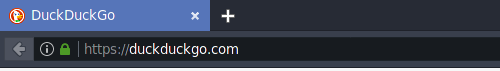
\includegraphics[scale=1]{Duck.png}\\
		\footnotesize O cadeado verde representa o certíficado SSL
	\end{center}

	O certíficado SSL nem sempre está nos sites, principalmente em sites pequenos, é comum eles não terem um certíficado SSL. Mas caso aconteça de algum site importante, como o site do Facebook ou o site do teu banco não tenha certíficado SSL, é recomendavel não fazer login.\\

	Os \href{https://criptowiki.miraheze.org/wiki/Spam}{spam} foram um método muito utilizado como forma de espalhar malwares e também para poder fazer phishing em usuários.\\

	Os spams são basicamente mensagens enviada para e-mails aleatórios com algum link para o usuário acessar ou algum arquivo para baixar. Eles foram e ainda é bem comum, embora não seja um método muito eficaz atualmente, mas caso receba alguma mensagem por e-mail com um título sensacionalista, é recomendavel não abri-lo. Então a dica é que antes de abrir uma mensagem de e-mail, pense 2 vezes ao abri-lo e se abrir, pense bem antes de clicar em algo.\\


\end{document}
